\section{Mediciones}

Se realizaron mediciones en base a crear arreglos de diferentes largos con
valores de energ\'ia consumida por entrenamiento y energ\'ias disponibles en el
rango de $[1,100]$ (como en los casos de prueba provistos por la catedra),
yendo de 10 en 10 elementos, donde los elementos en cada caso fueron generados
por los valores pseudoaleatorios del lenguaje (el m\'odulo \texttt{random}).

\begin{figure}[H]
    \centering % comparar el tiempo de ejecucion con (n^2)
    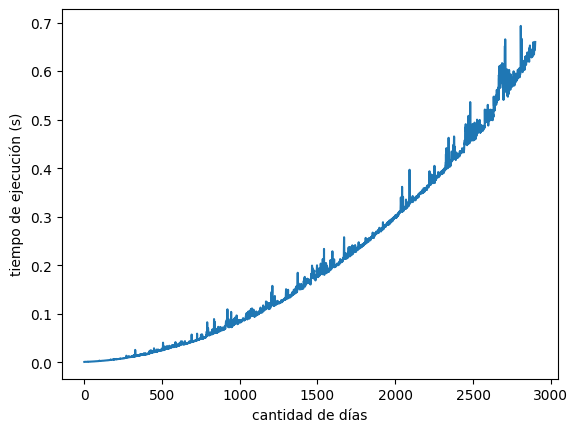
\includegraphics[width=1\textwidth]{img/tiempos.png}
\end{figure}

Como se puede apreciar, el algoritmo tiende a $\mathcal{O}\left( n^2 \right)$.
